\section{Case Study\label{sec:casestudy}: visual exploration of topic modeling}

The Topic Model Web Tool (TMWT) helps non-experts to explore collections of
text documents using topic modeling and
visualization. Topic modeling~\cite{Blei:2003:LDA},
although powerful, often requires human guidance in both the 
data preprocessing step as well as the
interpretation of topics once a model is fit to the data.
%~\cite{Sievert:2014:LAM}.

\begin{figure*}
  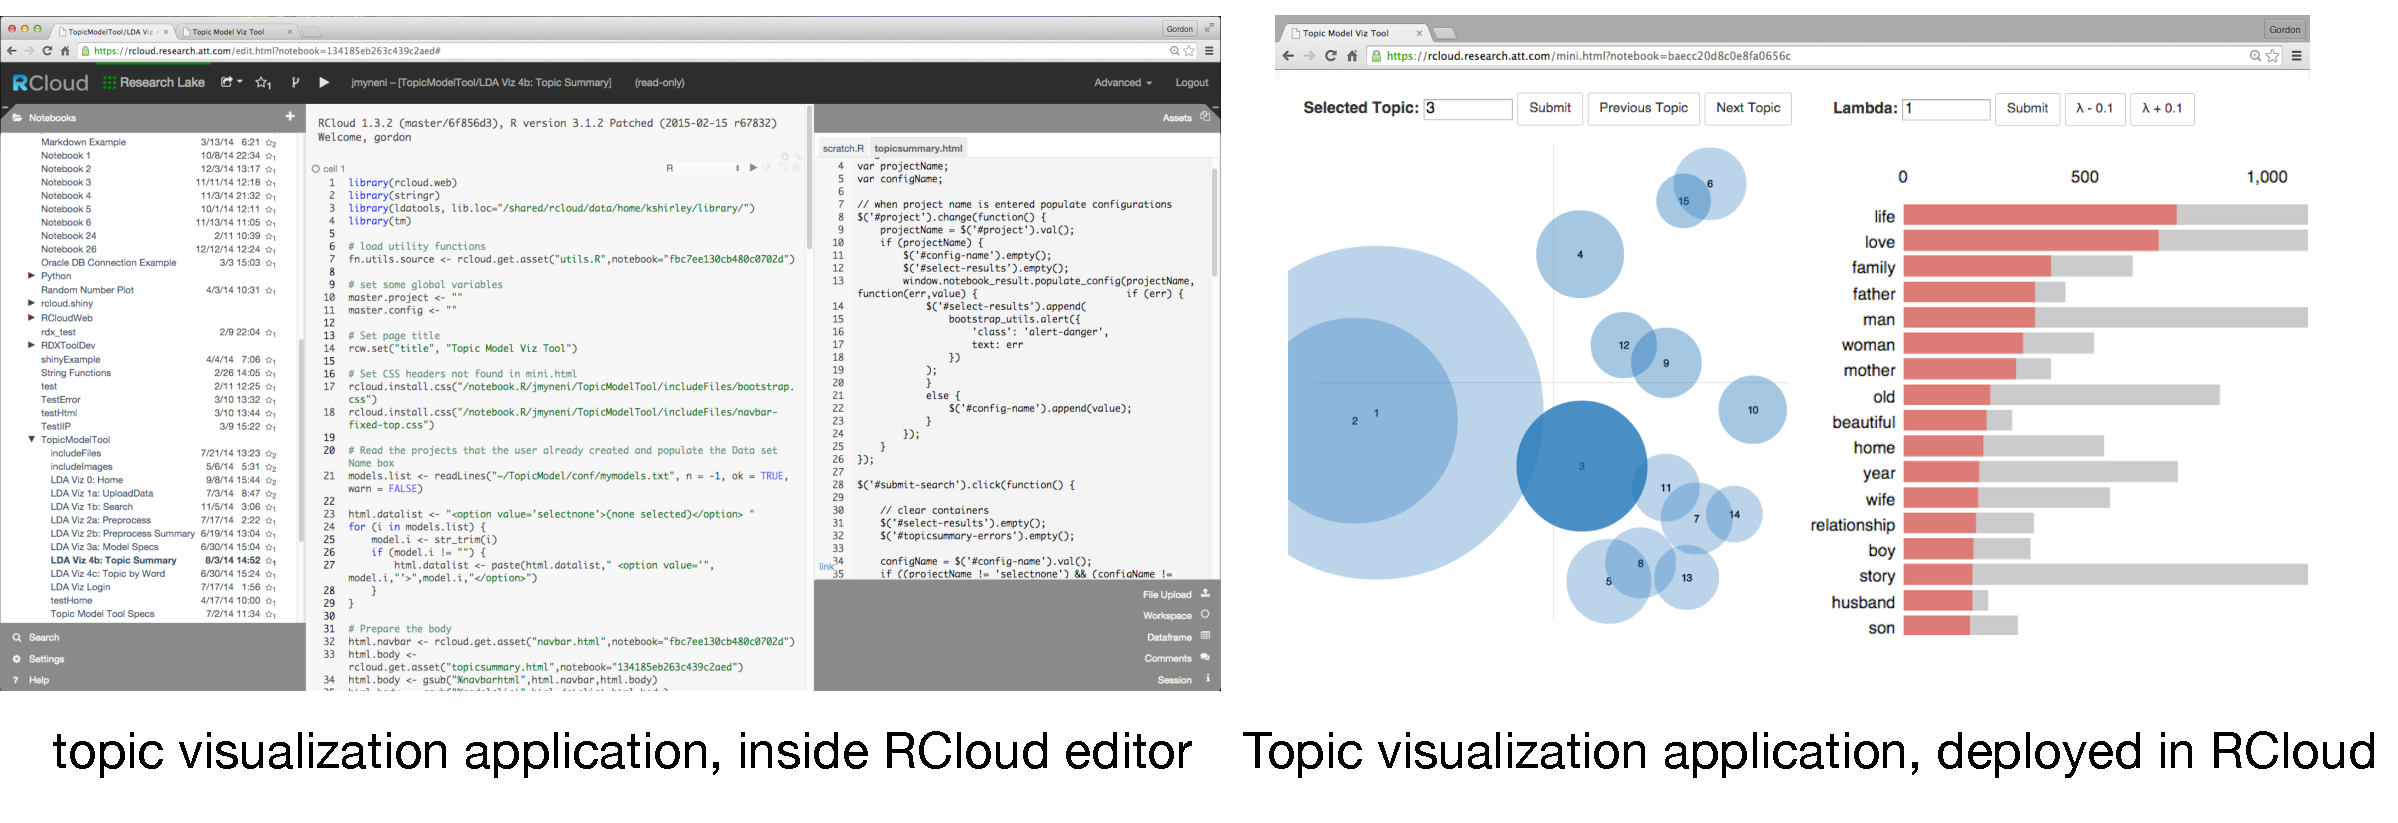
\includegraphics[width=\linewidth]{fig/casestudytext/casestudytext.pdf}
  \caption{\label{fig:textvis}The Topic Model Web Tool (TMWT), an example application developed
    and deployed entirely in RCloud.  TMWT allows analysts to
    fit and visually explore \emph{topic models}, statistical
    representations of different topics in a document collection.
  }
\end{figure*}

TMWT was developed by two technical staff members at
AT\&T Labs, originally in RStudio Shiny~\cite{RStudio:2013:SWA},
a framework for developing web applications in R.
While Shiny offers outstanding ease of development,
discoverability and deployment are also very important aspects
in an application's lifecycle (see Section~\ref{sec:interviews}).
RCloud's assumption that \emph{all developed notebooks are automatically
deployed} simplifies this for TMWT.

TMWT combines text preprocessing, topic modeling, and
interactive visualization. Text preprocessing is done
using standard string manipulation functions in R as well as
some functions from the tm package \cite{R:tm} to perform
such steps as global substitutions, tokenization, stop word removal, 
and stemming. Each of these preprocessing steps is controlled by the user
by allowing him/her to make selections in dropdown menu or, in 
some cases (such as defining the stop word list) uploading 
a custom file. Topic modeling is performed by
combining a standard R library to fit Latent Dirichlet 
Allocation (LDA) models using
Gibbs sampling with custom-developed R code. Last, the interactive
visualization of the fitted model is done using the LDAvis R package
\cite{R:LDAvis}, which aids topic interpretation.
The analysis module is a single R function
exposed to the web application via the Javascript-R RPC
mechanism described in Section~\ref{sec:system};
thus analysis is performed remotely on an RCloud server.

Each topic under LDA is a probability distribution over all the unique
words in the collection of documents. To expose patterns in the relationships
between topics, LDAVis combines
interactive visualization and dimensionality reduction,
allowing users to adjust measures for topic distances and the choice
of dimensionality reduction technique. The dimensionality reduction
algorithms and distance measures are implemented in R, which
means they can be executed on RCloud servers as well.

The result of the dimensionality reduction process in LDAvis is a
two-dimensional plot of the topic space, an example of which is shown in
Figure~\ref{fig:textvis}. The interactive view is implemented in SVG
and Javascript through D3~\cite{Bostock:2011:DDD}. One of the most
popular web-based visualization libraries for R is ggvis~\cite{ggvis},
so it is natural to ask if ggvis could have been used instead of
custom Javascript. In this case, the interactive features of ggvis
and Shiny are a subset of Vega's~\cite{vega}.
Custom interactions in LDAVis (like hovering over a topic or word, or adjusting the 
rankings of topic keywords) are not available yet in Vega~\cite{vega},
although the required components were recently described by Satyanarayan et
al.~\cite{Satyanarayan:2014:DID}.
Although LDAVis required custom Javascript, that flexibility is welcomed
by many web developers.

LDAVis demonstrates some unique features of RCloud.
While RCloud notebooks allow deployment of analyses over
the web with no extra effort, RCloud \emph{applications} are more
powerful, and are developed by combining Javascript and HTML
for the front end. This requires more expertise than Shiny, but
the RCloud model makes analysis simpler (since analysts
simply write R in the style they already know)
and the visualization front end is simpler for web
developers (since they simply write Javascript in
the style \emph{they} know).
LDAVis inherits the automatic deployment and discoverability
of all RCloud applications.
% In addition, RCloud applications
% inherit the automatic deployment and discoverability features of
% all RCloud notebooks.

% IMPORTANT: what is unique about RCloud here
% From prototyping to dashboard
% Getting other information from the web
%
